% The Klee--Minty square for n=2 (generated by figs_c2ch07.py).
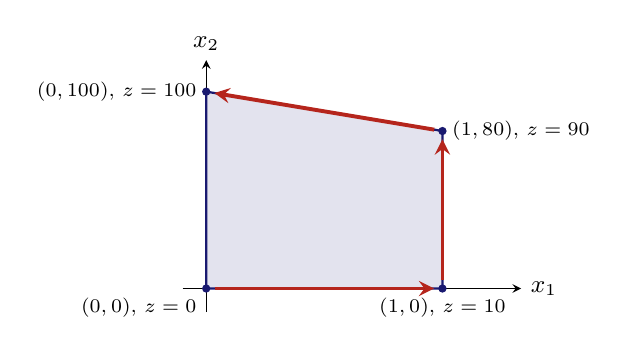
\begin{tikzpicture}[x=1cm,y=1cm,every node/.style={font=\small},>=stealth]
\draw[->] (-0.3,0) -- (4,0) node[right] {$x_1$};
\draw[->] (0,-0.3) -- (0,2.9) node[above] {$x_2$};
\fill[MidnightBlue!12] (0.0,0.0) -- (3.0,0.0) -- (3.0,2.0) -- (0.0,2.5) -- cycle;
\draw[MidnightBlue,thick] (0.0,0.0) -- (3.0,0.0) -- (3.0,2.0) -- (0.0,2.5) -- cycle;
\fill[MidnightBlue] (0.0,0.0) circle (1.5pt);
\node[below left,font=\scriptsize] at (0.0,0.0) {$(0,0)$, $z=0$};
\fill[MidnightBlue] (3.0,0.0) circle (1.5pt);
\node[below,font=\scriptsize] at (3.0,0.0) {$(1,0)$, $z=10$};
\fill[MidnightBlue] (3.0,2.0) circle (1.5pt);
\node[right,font=\scriptsize] at (3.0,2.0) {$(1,80)$, $z=90$};
\fill[MidnightBlue] (0.0,2.5) circle (1.5pt);
\node[left,font=\scriptsize] at (0.0,2.5) {$(0,100)$, $z=100$};
\draw[->,line width=1.4pt,BrickRed,shorten >=3pt,shorten <=3pt] (0.0,0.0) -- (3.0,0.0);
\draw[->,line width=1.4pt,BrickRed,shorten >=3pt,shorten <=3pt] (3.0,0.0) -- (3.0,2.0);
\draw[->,line width=1.4pt,BrickRed,shorten >=3pt,shorten <=3pt] (3.0,2.0) -- (0.0,2.5);
\end{tikzpicture}
